\normaltrue
\correctionfalse

%\UPSTIidClasse{12} % 11 sup, 12 spé
%\newcommand{\UPSTIidClasse}{12}

\exer{Barrière Sympact  $\star$ \label{C2:091D:14}}
\setcounter{question}{0}\UPSTIcompetence[2]{C2-09}
\index{Compétence C2-09}
\index{Principe fondamental de la dynamique}
\index{PFD}
\index{Mécanisme à 1 rotation}
\index{Barrière Sympact}
\ifcorrection
\else
\textbf{Pas de corrigé pour cet exercice.}
\fi

\ifprof
\else

La barrière Sympact permet d'ouvrir ou de fermer l'accès à un parking.

\begin{center}
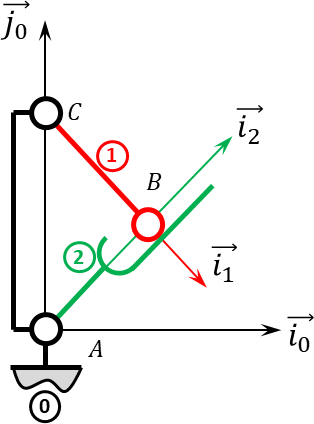
\includegraphics[width=\linewidth]{14_01}
\end{center}

L'angle d'ouverture est de  est $\alpha  = 90\degres$. La durée d'ouverture et de fermeture doit être $T=\SI{1}{s}$ au maximum. L'accélération maximale est de $\ddot{\theta}_{\text{max}}=\SI{30}{rad.s^{-2}}$.
La loi d'évolution est un trapèze de vitesse. On note$t_a$ le temps d'accélération (égal au temps de décélération) et $T$ le temps passé à vitesse constante. On note $\dot{\theta}_{\text{max}}$ la vitesse angulaire maximale. 

\fi


\question{Donner \textbf{l'allure} des lois d'accélération, vitesse et position angulaires. Vous indiquerez toutes les valeurs utiles (sous forme littérale). }
\ifprof
\else
\fi


\question{Donner l'expression littérale du temps total.}
\ifprof
\else
\fi

\question{Donner l'expression littérale de la vitesse angulaire en fin de phase d'accélération.}
\ifprof
\else
\fi



\question{Donner l'expression littérale de l'angle total parcouru.}
\ifprof
\else
\fi



\question{Déterminer la durée de l'accélération ainsi que la vitesse angulaire maximale atteinte.}
\ifprof
\else
\fi


\ifprof
\else
\begin{flushright}
\footnotesize{Corrigé  voir \ref{C2:091D:14}.}
\end{flushright}%
\fi